\chapter{Fundamentos del juego Onitama}
\label{chap:fundamentos-juego-onitama}

%==============================================================================
% 3.1. Descripción general del juego
% =============================================================================
\section{Descripción general del juego}
\label{sec:descripcion-general-onitama}

\textit{Onitama} es un juego de mesa abstracto de estrategia para dos jugadores, diseñado por Shimpei Sato y publicado originalmente en Japón en 2014. En este trabajo se toma como referencia la edición y el reglamento de Arcane Wonders, una de las editoriales principales en su distribución internacional \cite{onitama_bgg,onitama_rulebook}.

La propuesta del juego se basa en un enfrentamiento directo entre dos escuelas de artes marciales. Cada jugador controla a un maestro y a sus discípulos sobre un tablero reducido, tratando de superar al rival mediante movimientos precisos y decisiones cuidadosamente planificadas. Esta premisa permite presentar el juego de forma sencilla, sin necesidad de una gran cantidad de piezas, reglas o excepciones.

El aspecto más característico de \textit{Onitama} es que los movimientos disponibles no dependen de cada pieza de forma individual, sino de un conjunto limitado de cartas visibles. Estas cartas cambian durante la partida, por lo que cada turno afecta tanto a la posición actual del tablero como a las opciones que estarán disponibles más adelante. Por ello, aunque el juego utiliza pocos elementos, cada decisión tiene consecuencias tácticas inmediatas y estratégicas a medio plazo.

Estas características hacen que \textit{Onitama} sea un caso adecuado para el sistema desarrollado en este trabajo, al combinar una estructura discreta, un funcionamiento por turnos y elementos físicos claramente observables. Por ello, en las siguientes secciones se describen los elementos que componen una partida, la configuración inicial, el desarrollo de los turnos, las condiciones de victoria y las implicaciones que estas reglas tienen sobre el sistema implementado.


%==============================================================================
% 3.2. Elementos y configuración inicial
% =============================================================================
\section{Elementos y configuración inicial}
\label{sec:elementos-configuracion-inicial}

\textit{Onitama} utiliza un conjunto reducido de componentes, lo que facilita la comprensión de la partida desde el primer momento. Los elementos principales son el tablero, las piezas de ambos jugadores y las cartas de movimiento.

\begin{itemize}
    \item \textbf{Tablero}: está formado por una cuadrícula de \(5 \times 5\) casillas. En la fila inicial de cada jugador existe una casilla especial, situada en el centro, denominada templo. Esta casilla interviene tanto en la colocación inicial del maestro como en una de las condiciones de victoria.

    \item \textbf{Piezas}: cada jugador dispone de cinco piezas de un mismo color: un maestro y cuatro estudiantes. Todas las piezas utilizan las mismas cartas de movimiento, por lo que el tipo de pieza no determina cómo se desplaza. No obstante, el maestro tiene una importancia especial dentro de los objetivos de la partida.

    \item \textbf{Cartas de movimiento}: el juego base incluye dieciséis cartas. Cada carta representa un patrón de desplazamientos posibles que puede aplicarse a cualquiera de las piezas del jugador activo. Estas cartas no pertenecen de forma permanente a un jugador, sino que rotan entre ambos durante la partida.
\end{itemize}

La configuración inicial se realiza a partir de estos elementos y determina la situación desde la que comienza la partida:

\begin{enumerate}
    \item Cada jugador coloca su maestro en la casilla de templo correspondiente.
    \item Los cuatro estudiantes se sitúan en las casillas restantes de esa misma fila, a los lados del maestro.
    \item Se barajan las dieciséis cartas de movimiento.
    \item Cada jugador recibe dos cartas visibles, que forman su mano inicial.
    \item Se revela una quinta carta, que se coloca en el lateral del tablero.
    \item El sello de color de esa quinta carta determina qué jugador realiza el primer turno.
    \item Las cartas restantes no se utilizan durante esa partida.
\end{enumerate}

La Figura~\ref{fig:configuracion-inicial-onitama} muestra de forma esquemática esta disposición inicial, incluyendo la posición de las piezas, las cartas visibles de cada jugador y la carta lateral.

\begin{figure}[htbp]
    \centering

    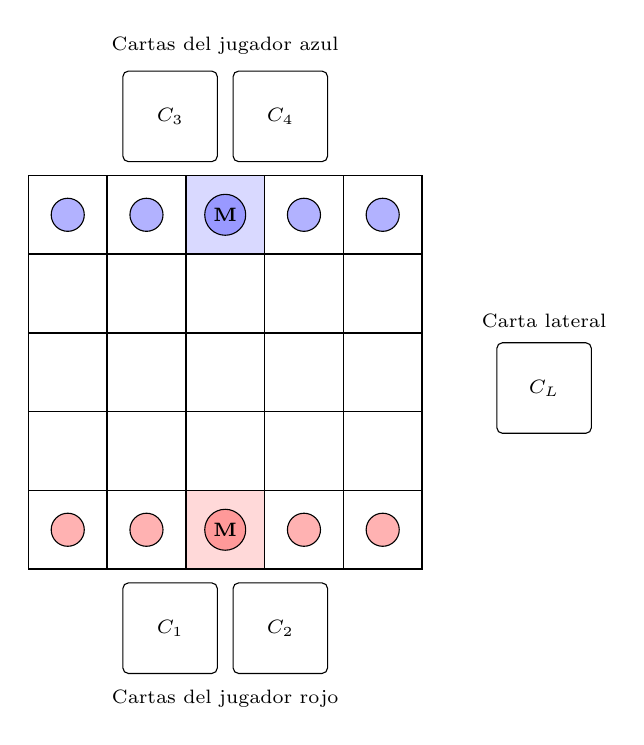
\begin{tikzpicture}[
        board/.style={
            line width=0.5pt
        },
        templeBlue/.style={
            fill=blue!15
        },
        templeRed/.style={
            fill=red!15
        },
        studentBlue/.style={
            circle,
            draw,
            fill=blue!30,
            minimum size=0.42cm,
            inner sep=0pt
        },
        studentRed/.style={
            circle,
            draw,
            fill=red!30,
            minimum size=0.42cm,
            inner sep=0pt
        },
        masterBlue/.style={
            circle,
            draw,
            fill=blue!40,
            minimum size=0.52cm,
            inner sep=0pt,
            font=\scriptsize\bfseries
        },
        masterRed/.style={
            circle,
            draw,
            fill=red!40,
            minimum size=0.52cm,
            inner sep=0pt,
            font=\scriptsize\bfseries
        },
        card/.style={
            rectangle,
            draw,
            rounded corners=2pt,
            fill=white,
            minimum width=1.20cm,
            minimum height=1.15cm,
            font=\scriptsize
        },
        labelText/.style={
            font=\scriptsize
        }
    ]

        \node[labelText] at (2.5,6.65) {Cartas del jugador azul};
        \node[card] at (1.8,5.75) {$C_3$};
        \node[card] at (3.2,5.75) {$C_4$};

        \node[labelText] at (6.55,3.15) {Carta lateral};
        \node[card] at (6.55,2.30) {$C_L$};

        \fill[templeRed] (2,0) rectangle (3,1);
        \fill[templeBlue] (2,4) rectangle (3,5);

        \draw[board] (0,0) rectangle (5,5);
        \foreach \i in {1,2,3,4} {
            \draw[board] (\i,0) -- (\i,5);
            \draw[board] (0,\i) -- (5,\i);
        }

        \foreach \x in {0.5,1.5,3.5,4.5} {
            \node[studentBlue] at (\x,4.5) {};
        }
        \node[masterBlue] at (2.5,4.5) {M};

        \foreach \x in {0.5,1.5,3.5,4.5} {
            \node[studentRed] at (\x,0.5) {};
        }
        \node[masterRed] at (2.5,0.5) {M};

        \node[card] at (1.8,-0.75) {$C_1$};
        \node[card] at (3.2,-0.75) {$C_2$};
        \node[labelText] at (2.5,-1.65) {Cartas del jugador rojo};

    \end{tikzpicture}

    \caption{Representación esquemática de la configuración inicial de una partida de \textit{Onitama}. Las casillas coloreadas de la columna central corresponden a los templos de cada jugador.}
    \label{fig:configuracion-inicial-onitama}
\end{figure}


%==============================================================================
% 3.3. Desarrollo de una partida
% =============================================================================
\section{Desarrollo de una partida}
\label{sec:desarrollo-partida-onitama}

Una vez establecida la configuración inicial, la partida avanza mediante turnos alternos. En cada turno, el jugador activo debe realizar dos pasos principales: primero mueve una de sus piezas utilizando una carta de movimiento y, después, intercambia la carta utilizada por la carta situada en el lateral del tablero \cite{onitama_rulebook}.

\subsubsection*{Movimiento y ataque}

El primer paso del turno consiste en elegir una de las dos cartas disponibles y aplicar uno de sus movimientos a una pieza propia. La pieza seleccionada puede ser tanto el maestro como cualquiera de los estudiantes, ya que en \textit{Onitama} los desplazamientos no dependen del tipo de pieza, sino de la carta utilizada.

Las cartas representan movimientos relativos respecto a la posición actual de la pieza. En cada carta, la casilla central indica la posición de origen y las casillas marcadas muestran los posibles destinos. Además, el patrón debe interpretarse desde la perspectiva del jugador que realiza el movimiento, por lo que una misma carta puede producir desplazamientos opuestos para cada jugador.

Para que un movimiento sea legal, deben cumplirse las siguientes condiciones:

\begin{itemize}
    \item La casilla de destino debe encontrarse dentro de los límites del tablero.
    \item La casilla de destino no puede estar ocupada por una pieza propia.
    \item El desplazamiento debe corresponderse con una de las posiciones indicadas por la carta seleccionada.
\end{itemize}

Si la casilla de destino está ocupada por una pieza rival, dicha pieza es capturada y se retira del tablero. Las piezas situadas entre la casilla de origen y la de destino no bloquean el movimiento, ya que el desplazamiento se considera directo. Del mismo modo, solo se captura una pieza rival cuando la pieza movida termina exactamente sobre su casilla.

\subsubsection*{Intercambio de cartas}

Después de resolver el movimiento, el jugador debe intercambiar la carta que acaba de utilizar. La carta usada se coloca en el lateral del tablero, orientada hacia el jugador contrario, y el jugador activo toma la carta que se encontraba previamente en esa posición. A partir de ese momento, dicha carta pasa a formar parte de sus opciones disponibles para turnos posteriores.

Este intercambio es una de las mecánicas más características de \textit{Onitama}. Cada turno no solo modifica la posición de las piezas, sino también el conjunto de cartas que estarán disponibles más adelante. Por tanto, una decisión puede ser favorable por el movimiento que permite en ese instante, pero también debe valorarse por la carta que entrega al rival.

Existe además un caso especial: si el jugador activo no puede realizar ningún movimiento legal con ninguna de sus dos cartas, debe pasar el turno. No obstante, incluso en esta situación debe escoger una de sus cartas e intercambiarla por la carta lateral, de manera que la circulación de cartas continúa aunque ninguna pieza se desplace \cite{onitama_rulebook}.


%==============================================================================
% 3.4. Condiciones de victoria
% =============================================================================
\section{Condiciones de victoria}
\label{sec:condiciones-victoria-onitama}

La partida finaliza cuando uno de los jugadores cumple una de las dos condiciones de victoria definidas por el reglamento. Ambas condiciones están relacionadas con el maestro, lo que diferencia a esta pieza del resto y le otorga un papel central dentro de la estrategia del juego \cite{onitama_rulebook}.

Las dos formas de ganar son las siguientes:

\begin{itemize}
    \item \textbf{Captura del maestro rival}: un jugador gana si una de sus piezas termina su movimiento sobre la casilla ocupada por el maestro del oponente. Esta condición es denominada en el reglamento como \textit{Way of the Stone}.
    
    \item \textbf{Llegada al templo contrario}: un jugador también gana si consigue mover su propio maestro hasta la casilla de templo del oponente. Esta condición es denominada en el reglamento como \textit{Way of the Stream}.
\end{itemize}

Estas dos vías de victoria generan objetivos complementarios. Por un lado, cada jugador debe proteger a su maestro para evitar una derrota inmediata por captura. Por otro lado, también puede buscar una victoria posicional avanzando con su maestro hasta el templo rival. Los estudiantes no activan directamente la victoria por templo, pero resultan importantes para controlar casillas, bloquear opciones del oponente y apoyar tanto la defensa como el avance del maestro.


%==============================================================================
% 3.5. Implicaciones para el sistema desarrollado
% =============================================================================
\section{Implicaciones para el sistema desarrollado}
\label{sec:implicaciones-sistema-onitama}

Las reglas descritas en las secciones anteriores condicionan directamente el diseño del sistema desarrollado. Al tratarse de un juego por turnos, con tablero discreto, piezas diferenciadas y cartas visibles, la aplicación debe coordinar varios módulos: motor de juego, inteligencia artificial, visión por computador e integración con la partida física.

Desde el punto de vista del motor de juego, una posición de \textit{Onitama} no queda definida únicamente por la colocación de las piezas sobre el tablero. También es necesario conocer qué jugador debe mover, qué cartas tiene disponibles cada jugador y qué carta se encuentra en el lateral. Por tanto, el estado de la partida debe integrar información espacial, información relativa a las piezas e información asociada a las cartas.

De forma resumida, el motor debe contemplar los siguientes aspectos:

\begin{itemize}
    \item La ocupación de cada una de las \(25\) casillas del tablero.
    \item El color y el tipo de cada pieza, diferenciando entre maestro y estudiantes.
    \item El jugador al que corresponde realizar el turno.
    \item Las dos cartas disponibles para cada jugador.
    \item La carta situada en el lateral.
    \item La generación de movimientos legales a partir de las cartas disponibles.
    \item La aplicación de capturas, intercambios de cartas y cambios de turno.
    \item La detección de las condiciones de victoria.
\end{itemize}

En el caso de la inteligencia artificial, estas reglas determinan el conjunto de acciones que puede analizar en cada turno. Las acciones legales generadas por el motor forman las alternativas de búsqueda, mientras que las condiciones de victoria permiten identificar estados terminales. Además, la importancia del maestro y la rotación de cartas influyen en la valoración estratégica de cada posición, ya que una jugada no solo debe evaluarse por el movimiento inmediato que produce, sino también por las cartas que deja disponibles para turnos posteriores.

Desde el punto de vista de la visión por computador, el sistema debe extraer del tablero físico la información necesaria para reconstruir una situación de partida válida. Esto implica identificar qué casillas están ocupadas, a qué jugador pertenece cada pieza, si se trata de un maestro o de un estudiante, y qué cartas se encuentran visibles en la disposición de la partida.

Por último, la integración entre visión, motor de reglas e inteligencia artificial exige comprobar que las observaciones obtenidas desde la cámara sean coherentes con la evolución legal del juego. No basta con detectar una configuración aislada del tablero, sino que es necesario verificar que el cambio observado respecto al estado anterior corresponde a una acción válida. Esta validación permite reducir errores derivados del ruido visual, de oclusiones temporales o de movimientos incompletos del jugador humano.

Estas implicaciones sirven como punto de partida para el análisis y diseño del sistema, que se aborda en el siguiente capítulo.
